\documentclass[12pt,a4paper]{article}
\usepackage{graphicx}
\usepackage{wrapfig}

\title{Praktikum Physik - Erzwungene Schwingungen}
\author{Simon Marti, Patricia Schwab, Mirco Kocher}
\date{09.03.2012}

\parindent=0pt 
\begin{document}
\maketitle

%%
% Ziel
%%
\section*{Ziel}
Messung der Eigenfrequenz der freien Schwingung bei unterschiedlichen D\"ampfungen und Bestimmung der D\"ampfungskonstante.

%%
% Motivation
%%
\section*{Motivation}
Der Versuch der erwungenen Schwingungen verschafft einen guten \"Uberblick \"uber das Gebiet der Differentalgleichungen. Ausserdem k\"onnen die gemessenen Daten graphisch auf logarithmischem Papier dargestellt werden. 

%%
% Theorie
%%
\section*{Theorie}
Die Periodendauer $T$ ist durch folgende Formel gegeben
\begin{equation}
T = \frac{Sekunden}{Perioden} \mbox [{s}]
\end{equation}
Die D\"ampfungskonstante $\alpha$ l\"asst sich durch folgende Formel absch\"atzen
\begin{equation}
\alpha = \frac{\ln\left( \frac{\varphi(n_{max} \cdot T)}{\varphi(n_{min} \cdot T)}\right)}{-T\cdot (n_{max} - n_{min})} \mbox [{s}^{-1}]
\end{equation}
Die Winkelgeschwindigkeit $\omega_0$ l\"asst sich folgendermassen bestimmen
\begin{equation}
\omega_0 = 2\pi \cdot T \mbox[{rad \cdot s}^{-1}]
\end{equation}
Ged\"ampfte harmonische Schwingung
\begin{equation}\label{eq:phi}
\varphi(t) = Ae^{-\alpha t}cos(\omega t - \beta)
\end{equation}
Die Resonanzfrequenz $\omega_0$ ist gegeben durch
\begin{equation}
\Omega_R = \sqrt{\omega_0^2 - 2\alpha^2} \mbox [{s}^{-1}]
\end{equation}
Die Resonanzkurve l\"asst sich durch folgende Formel beschreiben
\begin{equation}
A(\varepsilon) = \frac{M_0}{2J\omega_0\sqrt{\varepsilon^2 + \alpha^2}}
\end{equation}
wobei $\varepsilon = \Omega - \omega_0$, $J$ dem Tr\"agheitsmoment und $M_0$ dem Drehmoment entspricht.

\newpage

%%
% Experiment 1
%%
\section*{Experiment I}

% Aufbau und Ablauf
\subsection*{Aufbau und Ablauf}
Die Apparatur besteht aus einer vertikal stehenden Drehscheibe mit r\"ucktreibender Spiralfeder dessen Auslenkung an einer Skala abgelesen werden kann. Zwei Drahtspulen befinden sich beidseitig der Scheibe und wirken als Wirbelstrombremse deren St\"arke durch die Stromzufuhr geregelt werden kann. Ein Motor mit kontinuierlich verstellbarer Drehfrequenz liefert ein periodisches, externes Moment indem das feste Ende der Spiralfeder bewegt wird. Die Amplitude des Pendels wird jeweils von Patricia an der eingebauten Skala abgelesen, die Frequenz des Pendels und des Motors wird bestimmt indem Simon mir einer Stoppuhr zehn Perioden misst.

Beim ersten Experiment wird die Amplitude des Pendels in mehreren aufeinanderfolgenden Schwingungszyklen f\"ur verschiedene Dämpfungen gemessen. Das Pendel wurde jeweils bis zum Wert 9 auf der Skala ausgelenkt.

% Rohdaten
\subsection*{Rohdaten}
\subsubsection*{Ohne D\"ampfung}
Erste Messung

\vspace{3pt}
\begin{tabular}{|l|l|l|l|l|l|l|l|l|l|}
\hline
$A_{0}$&$A_{1}$&$A_{2}$&$A_{3}$&$A_{4}$&$A_{5}$&$A_{6}$&$A_{7}$&$A_{8}$&$A_{9}$\\
\hline
9.0&8.8&8.7&8.5&8.4&8.2&8.1&8.0&7.8&7.7\\
\hline
\hline
$A_{10}$&$A_{11}$&$A_{12}$&$A_{13}$&$A_{14}$&$A_{15}$&$A_{16}$&$A_{17}$&$A_{18}$&$A_{19}$\\
\hline
7.6&7.4&7.3&7.2&7.0&6.9&6.7&6.6&6.5&6.3\\
\hline
\hline
$A_{20}$&$A_{21}$&$A_{22}$&$A_{23}$&$A_{24}$&$A_{25}$&$A_{26}$&$A_{27}$&$A_{28}$&$A_{29}$\\
\hline
6.2&6.1&5.9&5.8&5.7&5.5&5.4&5.3&5.1&5.0\\
\hline
\end{tabular}

\vspace{10pt}
Zweite Messung

\vspace{3pt}
\begin{tabular}{|l|l|l|l|l|l|l|l|l|l|}
\hline
$A_{0}$&$A_{1}$&$A_{2}$&$A_{3}$&$A_{4}$&$A_{5}$&$A_{6}$&$A_{7}$&$A_{8}$&$A_{9}$\\
\hline
9.0&8.9&8.7&8.5&8.4&8.3&8.1&7.9&7.8&7.6\\
\hline
\hline
$A_{10}$&$A_{11}$&$A_{12}$&$A_{13}$&$A_{14}$&$A_{15}$&$A_{16}$&$A_{17}$&$A_{18}$&$A_{19}$\\
\hline
7.5&7.3&7.2&7.0&6.9&6.7&6.6&6.5&6.4&6.2\\
\hline
\hline
$A_{20}$&$A_{21}$&$A_{22}$&$A_{23}$&$A_{24}$&$A_{25}$&$A_{26}$&$A_{27}$&$A_{28}$&$A_{29}$\\
\hline
6.1&5.9&5.8&5.7&5.5&5.4&5.3&5.2&5.0&4.8\\
\hline
\end{tabular}

\vspace{10pt}
10$T$ = 20.0s

\subsubsection*{Mit D\"ampfung 0.45A}
Erste Messung

\vspace{3pt}
\begin{tabular}{|l|l|l|l|l|l|l|l|l|l|}
\hline
$A_{0}$&$A_{1}$&$A_{2}$&$A_{3}$&$A_{4}$&$A_{5}$&$A_{6}$&$A_{7}$&$A_{8}$&$A_{9}$\\
\hline
9.0&7.1&5.7&4.5&3.5&2.7&2.2&1.7&1.4&1.0\\
\hline
\end{tabular}
\vspace{10pt}

Zweite Messung

\vspace{3pt}
\begin{tabular}{|l|l|l|l|l|l|l|l|l|l|}
\hline
$A_{0}$&$A_{1}$&$A_{2}$&$A_{3}$&$A_{4}$&$A_{5}$&$A_{6}$&$A_{7}$&$A_{8}$&$A_{9}$\\
\hline
9.0&7.2&5.8&4.5&3.5&2.7&2.1&1.6&1.2&0.9\\
\hline
\end{tabular}

\vspace{10pt}
10$T$ = 20.0s

\subsubsection*{Mit D\"ampfung 0.6A}
Erste Messung

\begin{tabular}{|l|l|l|l|l|l|l|l|l|l|}
\hline
$A_{0}$&$A_{1}$&$A_{2}$&$A_{3}$&$A_{4}$&$A_{5}$&$A_{6}$&$A_{7}$&$A_{8}$&$A_{9}$\\
\hline
9.0&6.0&4.0&2.6&1.7&1.1&0.6&0.4&0.2&0.1\\
\hline
\end{tabular}
\vspace{10pt}

Zweite Messung

\vspace{3pt}
\begin{tabular}{|l|l|l|l|l|l|l|l|l|l|}
\hline
$A_{0}$&$A_{1}$&$A_{2}$&$A_{3}$&$A_{4}$&$A_{5}$&$A_{6}$&$A_{7}$&$A_{8}$&$A_{9}$\\
\hline
9.0&6.0&4.0&2.7&1.8&1.2&0.7&0.4&0.3&0.1\\
\hline
\end{tabular}

\vspace{10pt}
10$T$ = 20.0s

% Auswertung
\subsection*{Auswertung}
Der logaritmische zeitliche Verlauf von $\varphi(nT)$ l\"asst sich aus Gleichung \ref{eq:phi} bestimmen:
\[ ln(\varphi(nT)) = ln(Ae^{-\alpha nT}cos(\omega nT - \beta)) \]
\[ ln(\varphi(nT)) = ln(A) + ln(e^{-\alpha nT}) + ln(cos(\omega nT - \beta)) \]
\[ ln(\varphi(nT)) = ln(A) -\alpha nT + ln(cos(\omega nT - \beta)) \]
Nach Formel \ref{eq:omega}:
\[ \omega nT = 2\pi n \Rightarrow cos(\omega nT - \beta) = cos(- \beta) \]
\[ ln(\varphi(nT)) = \alpha nT + C \]
$\ln(\varphi(nT))$ ist linear, beschreibt also eine Gerade.

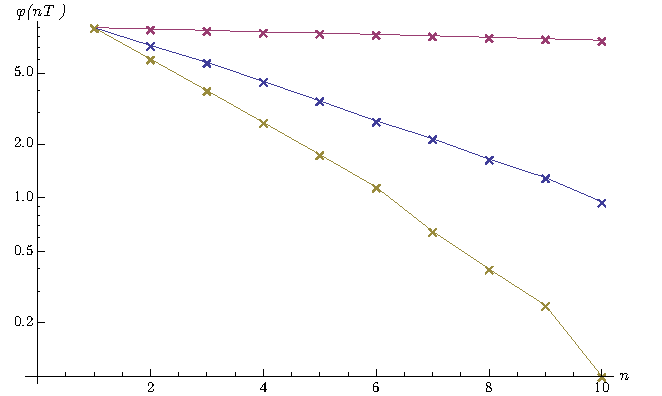
\includegraphics[width=15cm]{plot1.pdf}

% Zusammenfassung
\subsection*{Zusammenfassung}

%%
% Experiment 1I
%%
\section*{Experiment II}

% Aufbau und Ablauf
\subsection*{Aufbau und Ablauf}
Der Aufbau ist gleich wie bei Experiment I. Im Gegensatz zu Experiment I hat der Motor ein zus\"atzliches externes Moment geliefert. 
Zuerst haben wir die Resonanzfrequenz $\Omega_R$ mit der Abgesch\"atztung von $\alpha$ bestimmt. Dadurch konnten wir die maximale Amplitude bestimmen und in dieser Umgebung mehrere Punkte messen.
Dabei hat Patricia zus\"atzlich die Geschwindigkeit des Motors geregelt.

% Rohdaten
\subsection*{Rohdaten}
\subsubsection*{Ohne D\"ampfung}

\subsubsection*{Mit D\"ampfung 0.45A}

\subsubsection*{Mit D\"ampfung 0.6A}

% Auswertung
\subsection*{Auswertung}
Resonanzkurve

% Zusammenfassung
\subsection*{Zusammenfassung}
blupp

%%
% Experiment 1II
%%
\section*{Experiment III}

% Aufbau und Ablauf
\subsection*{Aufbau und Ablauf}
Die D\"ampfungskonstante $\alpha$ soll auf zwei verschiedene Arten bestimmt werden.\\
1. $\varphi(t) \approx e^{-\alpha t}$ \\
2. $\frac{A_{max}}{\sqrt{2}}$\\

% Auswertung
\subsection*{Auswertung}
blablaaa

% Zusammenfassung
\subsection*{Zusammenfassung}
blupp

%%
% Diskussion
%%
\section*{Diskussion}


\end{document}